\section{Milestone I}\label{M1}
In this section we want to study the evolution of the uniform background in the Universe. Our main goal of this section will be to implement methods that computes the Hubble parameter, as well as related time- and distance measures \note{Rewrite}. To do this, we will solve \note{simple} ordinary differential equations (ODEs) numerically. For the fiducial cosmology we will use results from \cite{Planck2020}. We will then test our implementation with known theoretical solutions, to assess the validity of our methods. 

The main goal of this section is mainly concerned with using known parameter values to \note{predict/solve} the background cosmology. Another interesting aspect is to use data to constrain such cosmological parameters. To do this, we will use data from supernova observations \cite{Supernova2014Betoule}, containing luminosity distance associated with different values of redshift. Implementing our solver, we will implement a simple Markov chain Monte Carlo (MCMC) algorithm, in order to estimate the best fits of $h,\,\Omega_m$ and $\Omega_\Lambda$, which are the Hubble parameter, and the density parameter of matter and dark energy, respectively.   


\subsection{Theory}\label{M1:theory}
The theory behind this milestone. 

When we don't assume $k=0$, the Friedmann equation can be written as 
\begin{equation}
    H = H_0 \sqrt{(\obn + \ocdmn)a^{-3} + (\ogn + \onun)a^{-4} + \okn a^{-2} + \oln} \label{M1:theory:eq:Friedmann_H_omegas}
\end{equation}
where $H\equiv\dot{a}/a$ is the Hubble parameter. 

\subsection{Implementation details}\label{M1:implementation} 
Something about the numerical work.

\subsection{Results}\label{M1:results}
Show and discuss the results.


\begin{figure}
    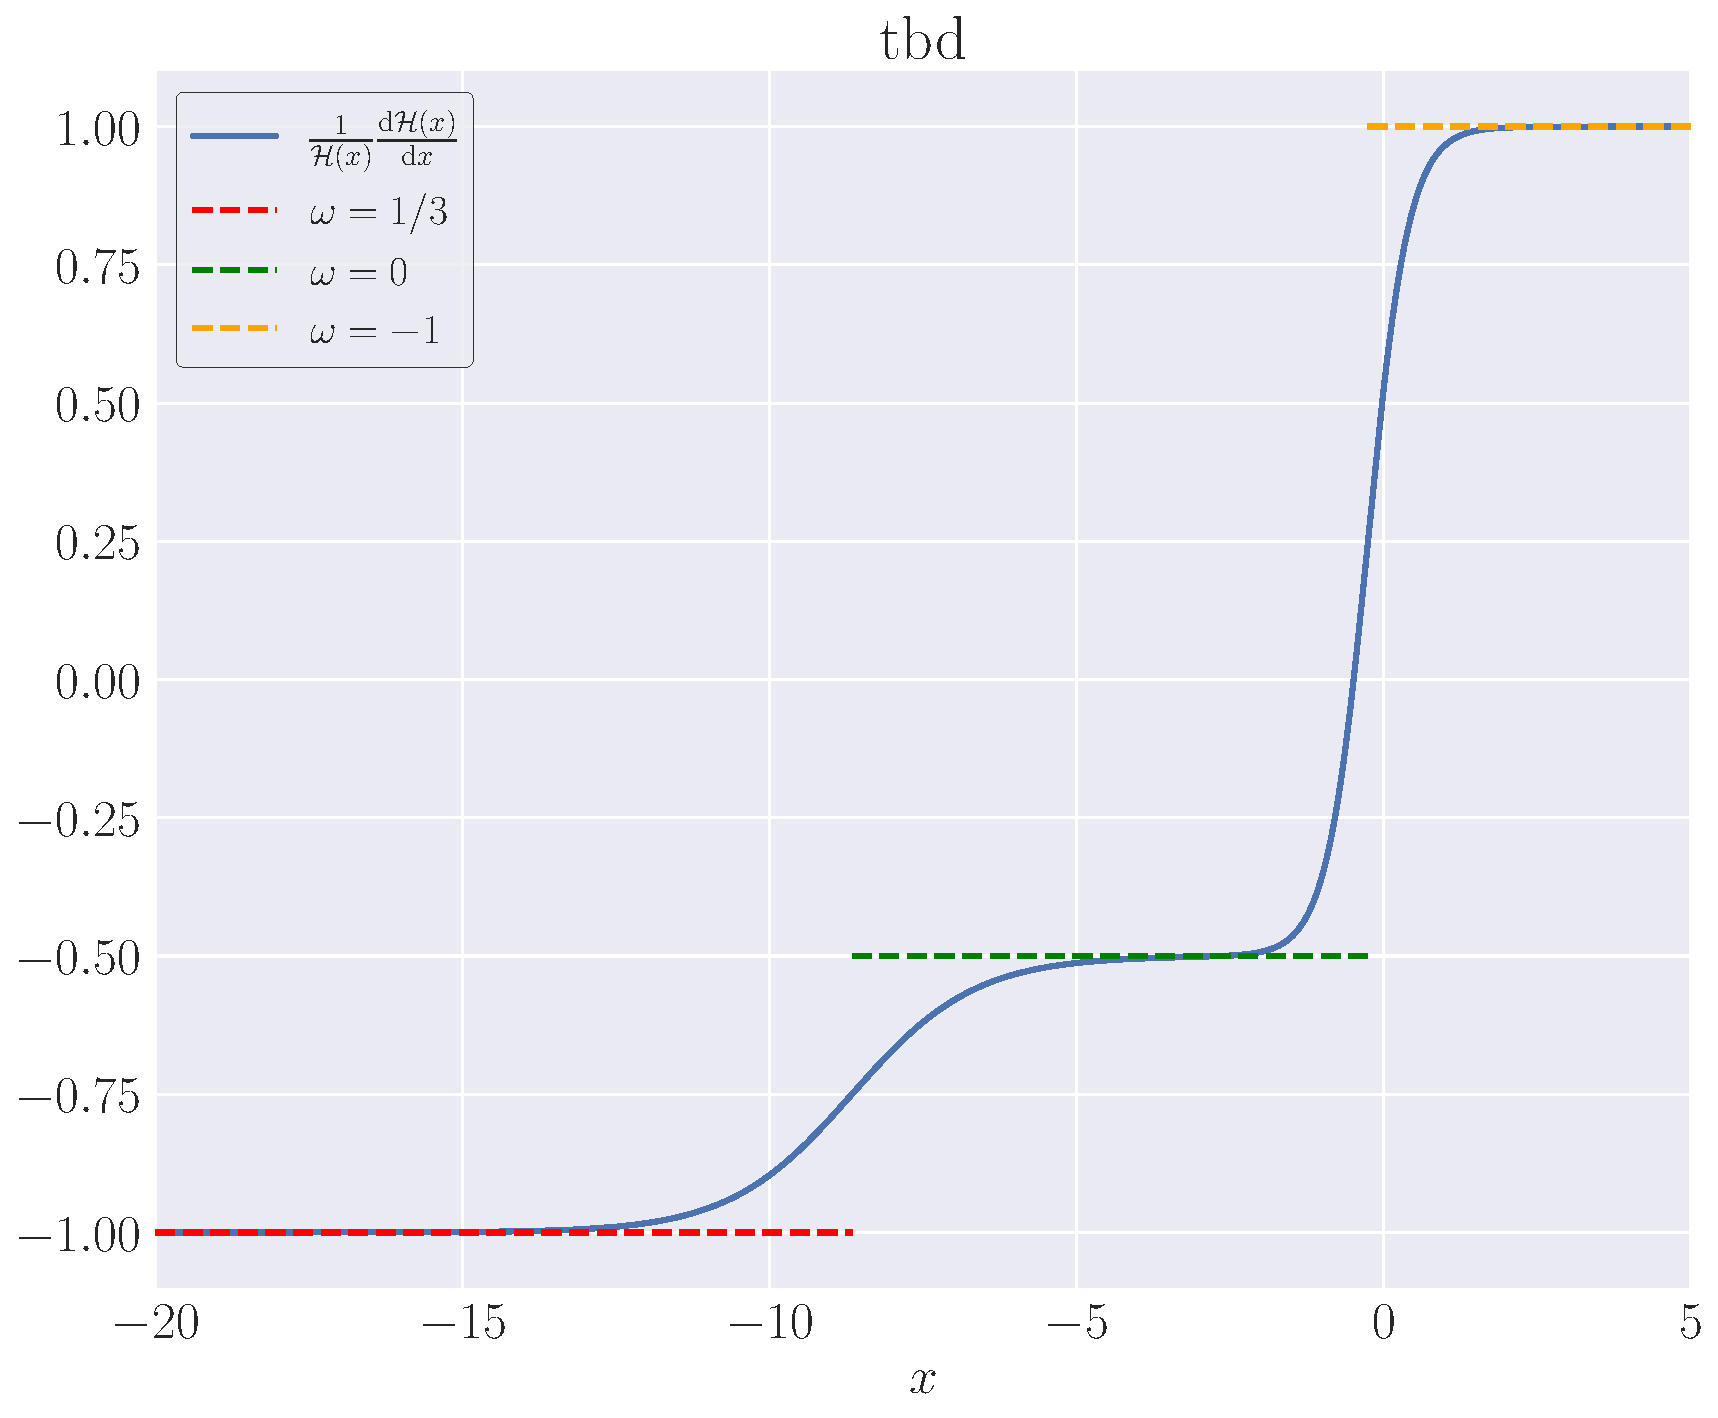
\includegraphics[width=\linewidth]{dH_over_H.pdf}
\end{figure}